% !TeX root = ./document.tex
\chapter{Reálné funkce, limita a spojitost}
Funkce z $M$ do $N$ je předpis, který každému prvku $M$ přiřadí nejvýše jeden \\ prvek z $N$
\begin{itemize}
    \item $A\subset M:f(A)=\left\{f(x); x\in A\right\}\subset N$
    \item $B\subset M:f^{-1}(B)=\left\{x\in M: f(x)\in B\right\}\subset M$
\end{itemize}

\begin{definition}[Prostá funkce, injekce, monomorfismus]\labelTheo{D-injection}
    Funkce je \textbf{prostá}, pokud $x\neq y \Rightarrow f(x)\neq f(y)$
\end{definition}

\begin{definition}[Na funkce, surjekce, epimorfismus]\labelTheo{D-surjection}
    Funkce $f:M\rightarrow N$ je \textbf{na} (zobrazuje $M$ na $N$), pokud
    $\forall n\in\mathbb{N}~\exists m\in M: f(m)=n$
    \begin{figure}[ht!]
        \begin{center}
            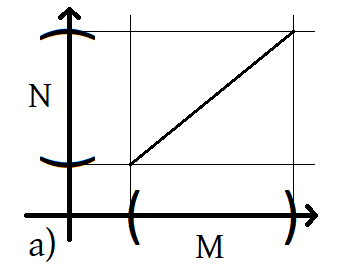
\includegraphics[width=0.4\textwidth,keepaspectratio]{../img/chapter2/surjectiveFunction.png}
            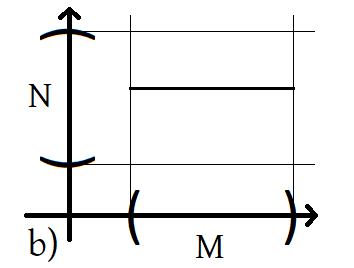
\includegraphics[width=0.4\textwidth,keepaspectratio]{../img/chapter2/surjectiveFunctionNOT.png}
            \caption{Funkce a) je na, funkce b) není.}
        \end{center}
    \end{figure}\FloatBarrier
    Př.: $\varphi$ není prostá, zobrazuje $\mathbb{R}$ na $[0,+\infty)$
    \begin{alignat}{1}
        \varphi:\mathbb{R}&\rightarrow\mathbb{R} \\
        x&\rightarrow x^2 \\
        \varphi((-1,1))&=[0,1)] \\
        \varphi^{-1}([1,4])&=[-2,-1]\cup[1,2]
    \end{alignat}
\end{definition}

\begin{definition}[vzájemně jednoznačné zobrazení, bijekce , isomorfismus]\labelTheo{D-bijection}
    Je-li $f:M\rightarrow N$ \hyperref[D-injection]{prostá} a \hyperref[D-surjection]{na} říkáme, že je vzájemně jednoznačná
\end{definition}

\begin{itemize}
    \item 

        $\Rightarrow$ lze definovat inverzní funkci:
        
        $f_{-1}:N\rightarrow M; y\in N\rightarrow \text{jediné }x\in M: f(x)=y$

        \[
        \textbf{Pozor!}
        \begin{cases}
            f^{-1} \quad\text{pro každou hodnotu zvlášť, je to množina} \\
            f_{-1} \quad\text{inverzní funkce}
        \end{cases}
        \]
    \item Je-li $f:M\rightarrow N$ a $A\subset M$: $f|_A$ nazvu restrikce (zúžení) $f$ na $A$
        
        Př.: $\varphi(x)=x^2: \varphi|_{[0,+\infty)}$ zobrazuje $[0,+\infty)$ na $[0,+\infty)$
        vzájemně jednoznačně. Lze tedy def $\varphi_{-1}=(\varphi|_{[0,+\infty)})_{-1}(x)=\sqrt{x}$
\end{itemize}

\begin{definition}[Složená funkce, superpozice]
    
\end{definition}